Upper limits are derived on the ratio of the product of the gluon fusion Higgs
boson production cross section by the H$\to \WW$ branching fraction,
$\sigma_{\rm{H}}~\cdot~$BR(H $\to \WW \to 2\ell2\nu)$ with respect to the
expected value in the SM for 1 $\ifb$ of integrated luminosity as benchmark point. 
We use a method is based on Bayesian 
inference~\cite{bayesian} to compute such limits, where we use a likelihood 
function from the expected number of observed events modeled as a Poisson 
random variable whose mean value is the sum of the contributions from signal 
and background processes. The method account for systematic uncertainties. 
Results are reported with a flat signal {\it prior}.To perform the
computation of the limits, the software package LandS is used.

The expected upper limits at 95\% C.L. for the cut based analysis are
shown in Figure~\ref{fig:cutbase_uls}. The expected upper limits at
95\% C.L. for the multivariate based analysis are shown in
Figure~\ref{fig:mvabase_uls} for a case where we apply a cut on the
discriminating variable and Figure~\ref{fig:mvashape_uls} where we use
the shape of the disciminating variable to maximize the analysis
sensitivity. The 

\begin{figure}[!htbp]
\begin{center}
   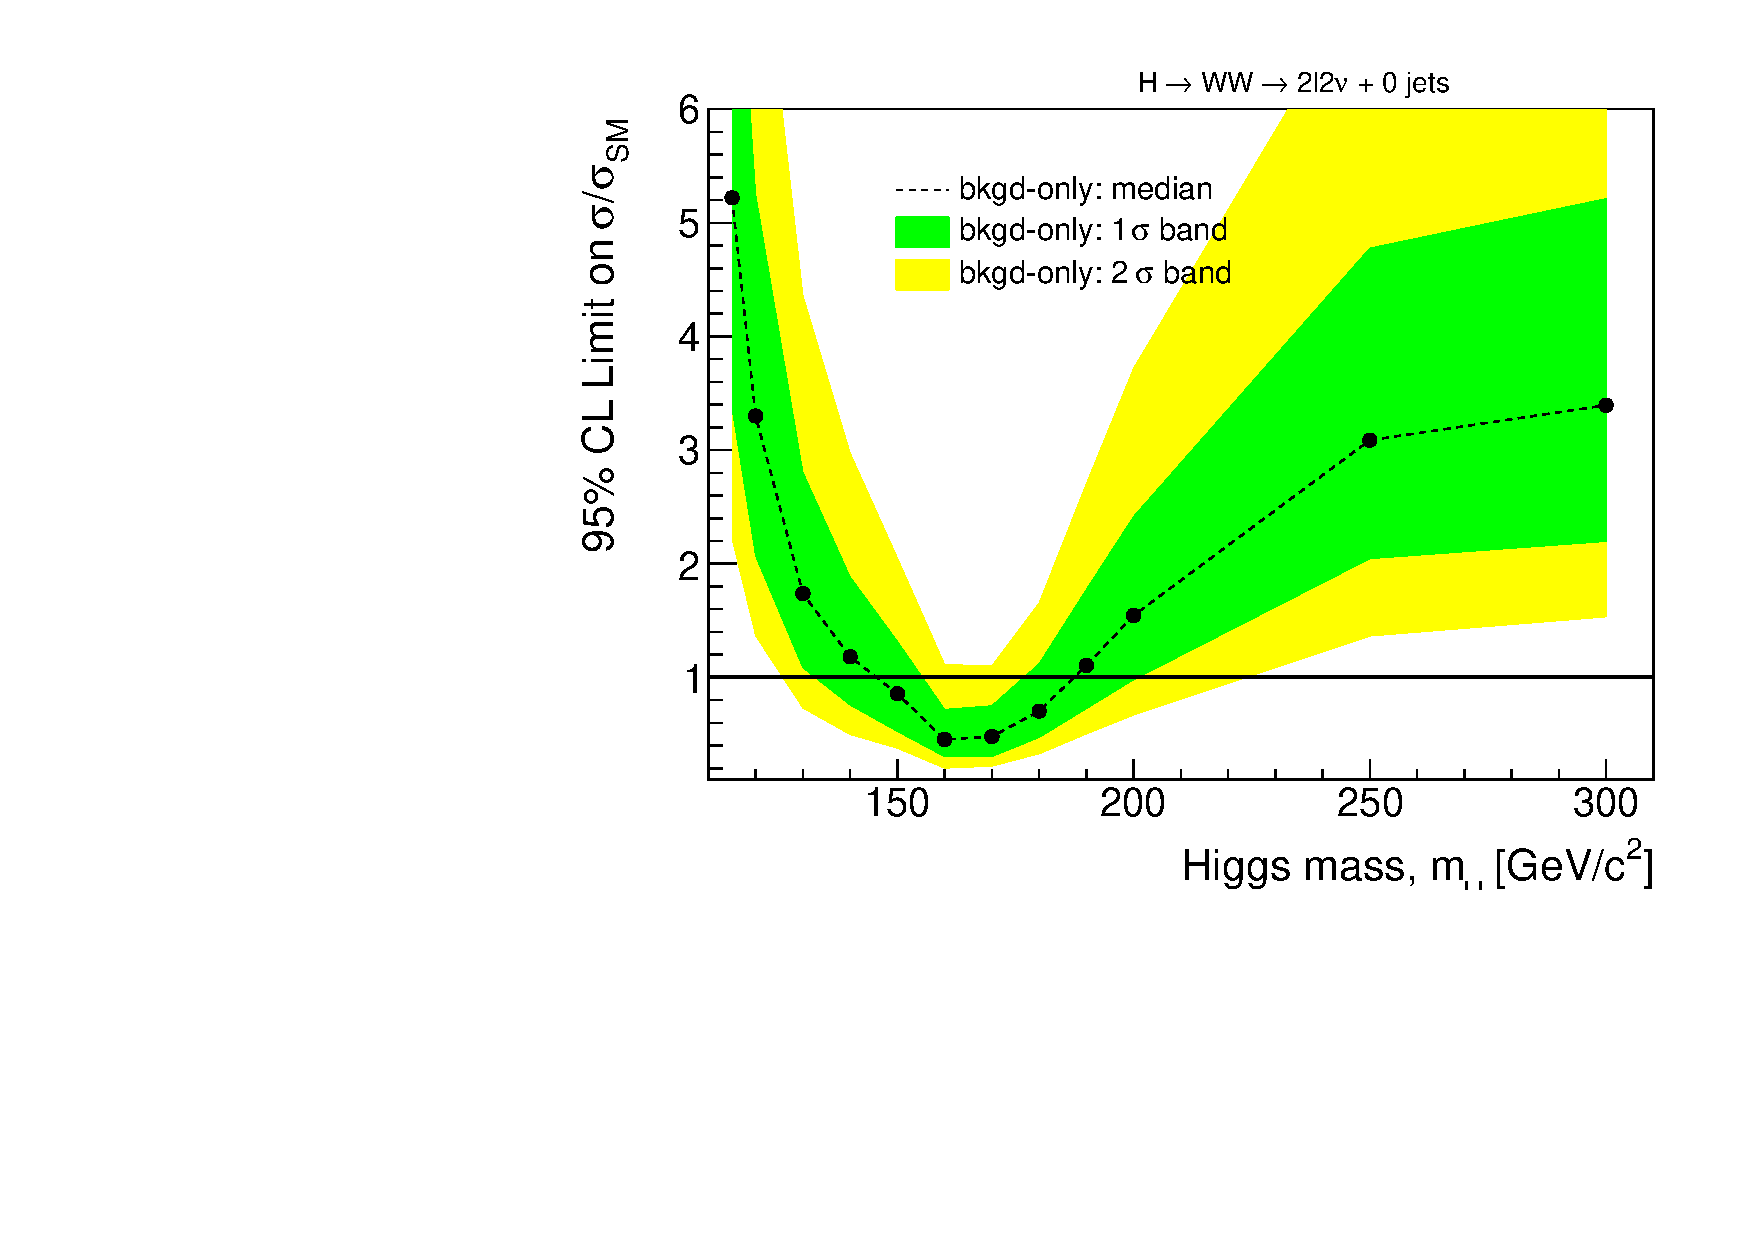
\includegraphics[width=0.49\textwidth]{figures/limits_0j_1000pb_cut_1.pdf}
   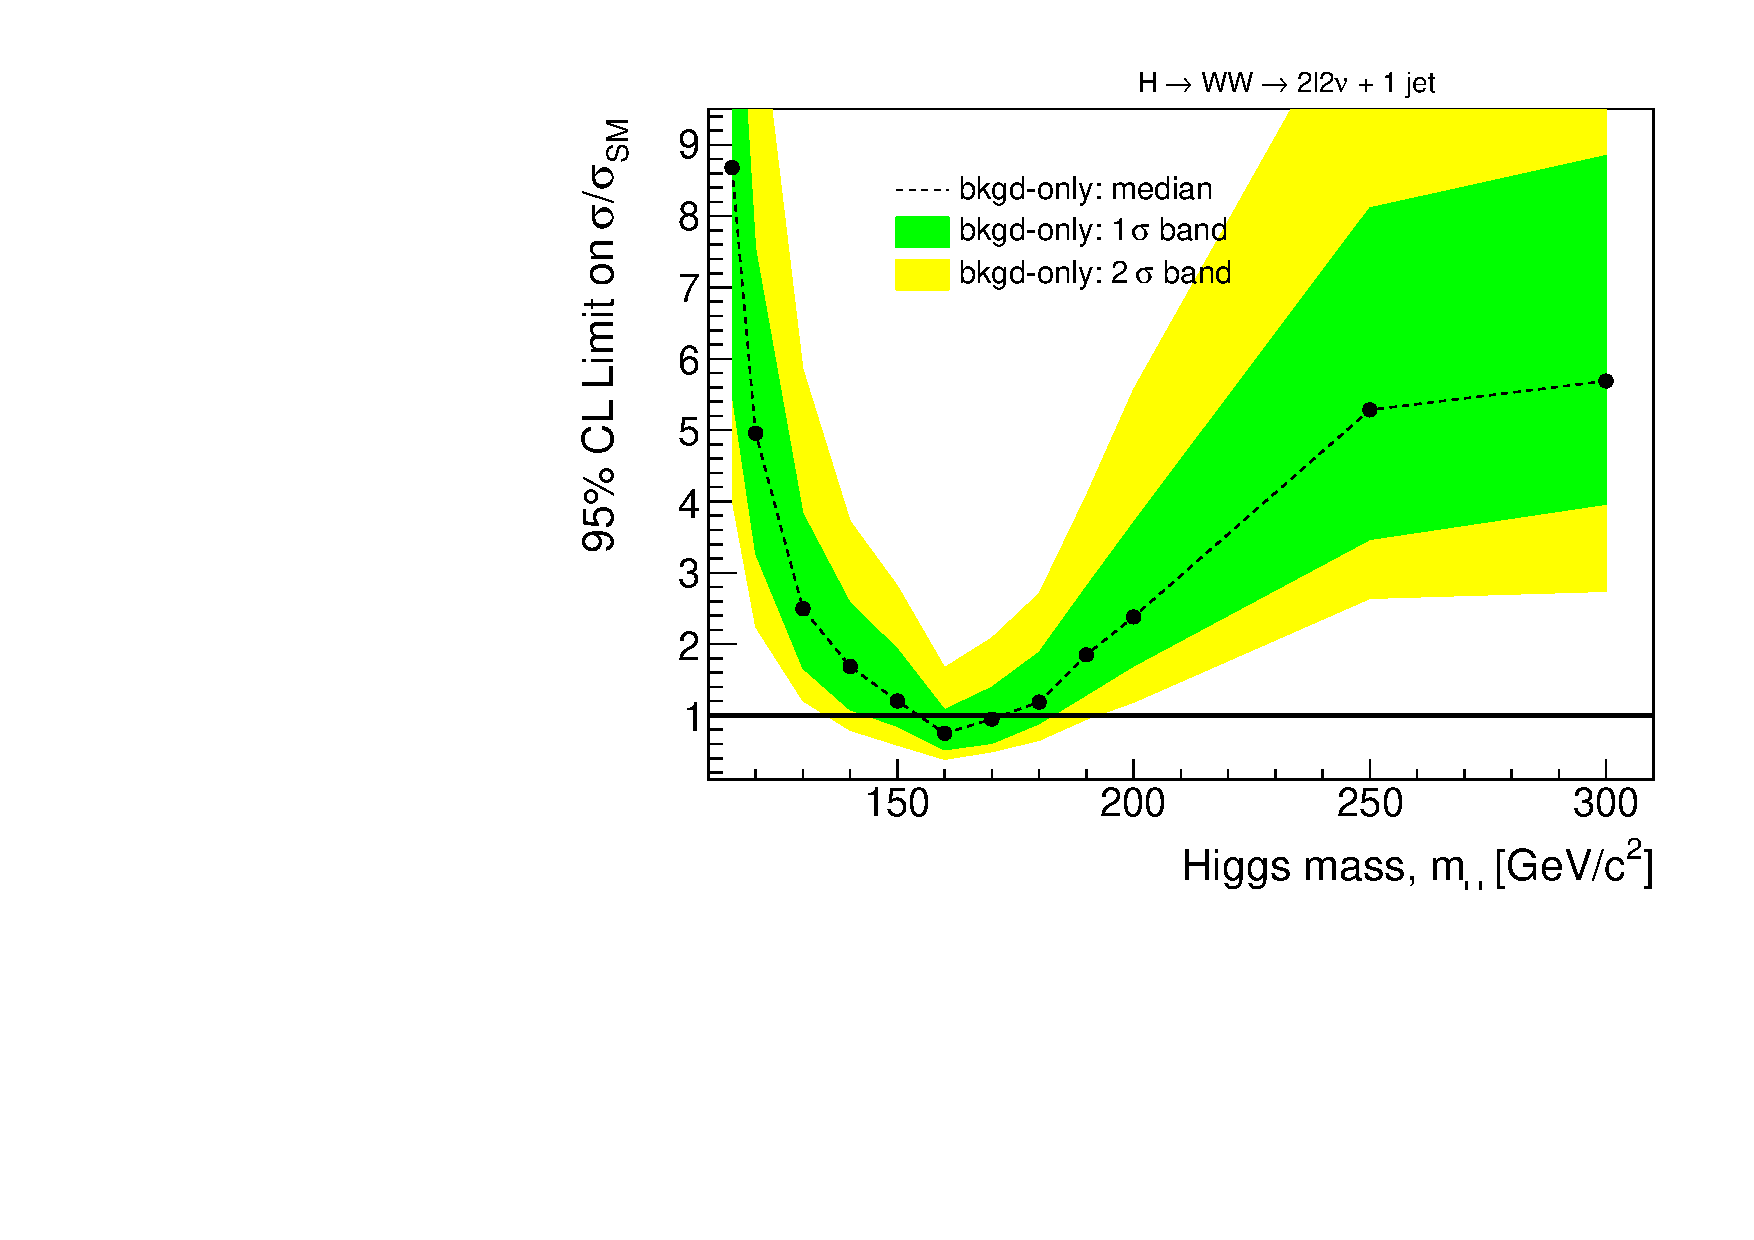
\includegraphics[width=0.49\textwidth]{figures/limits_1j_1000pb_cut_1.pdf}
   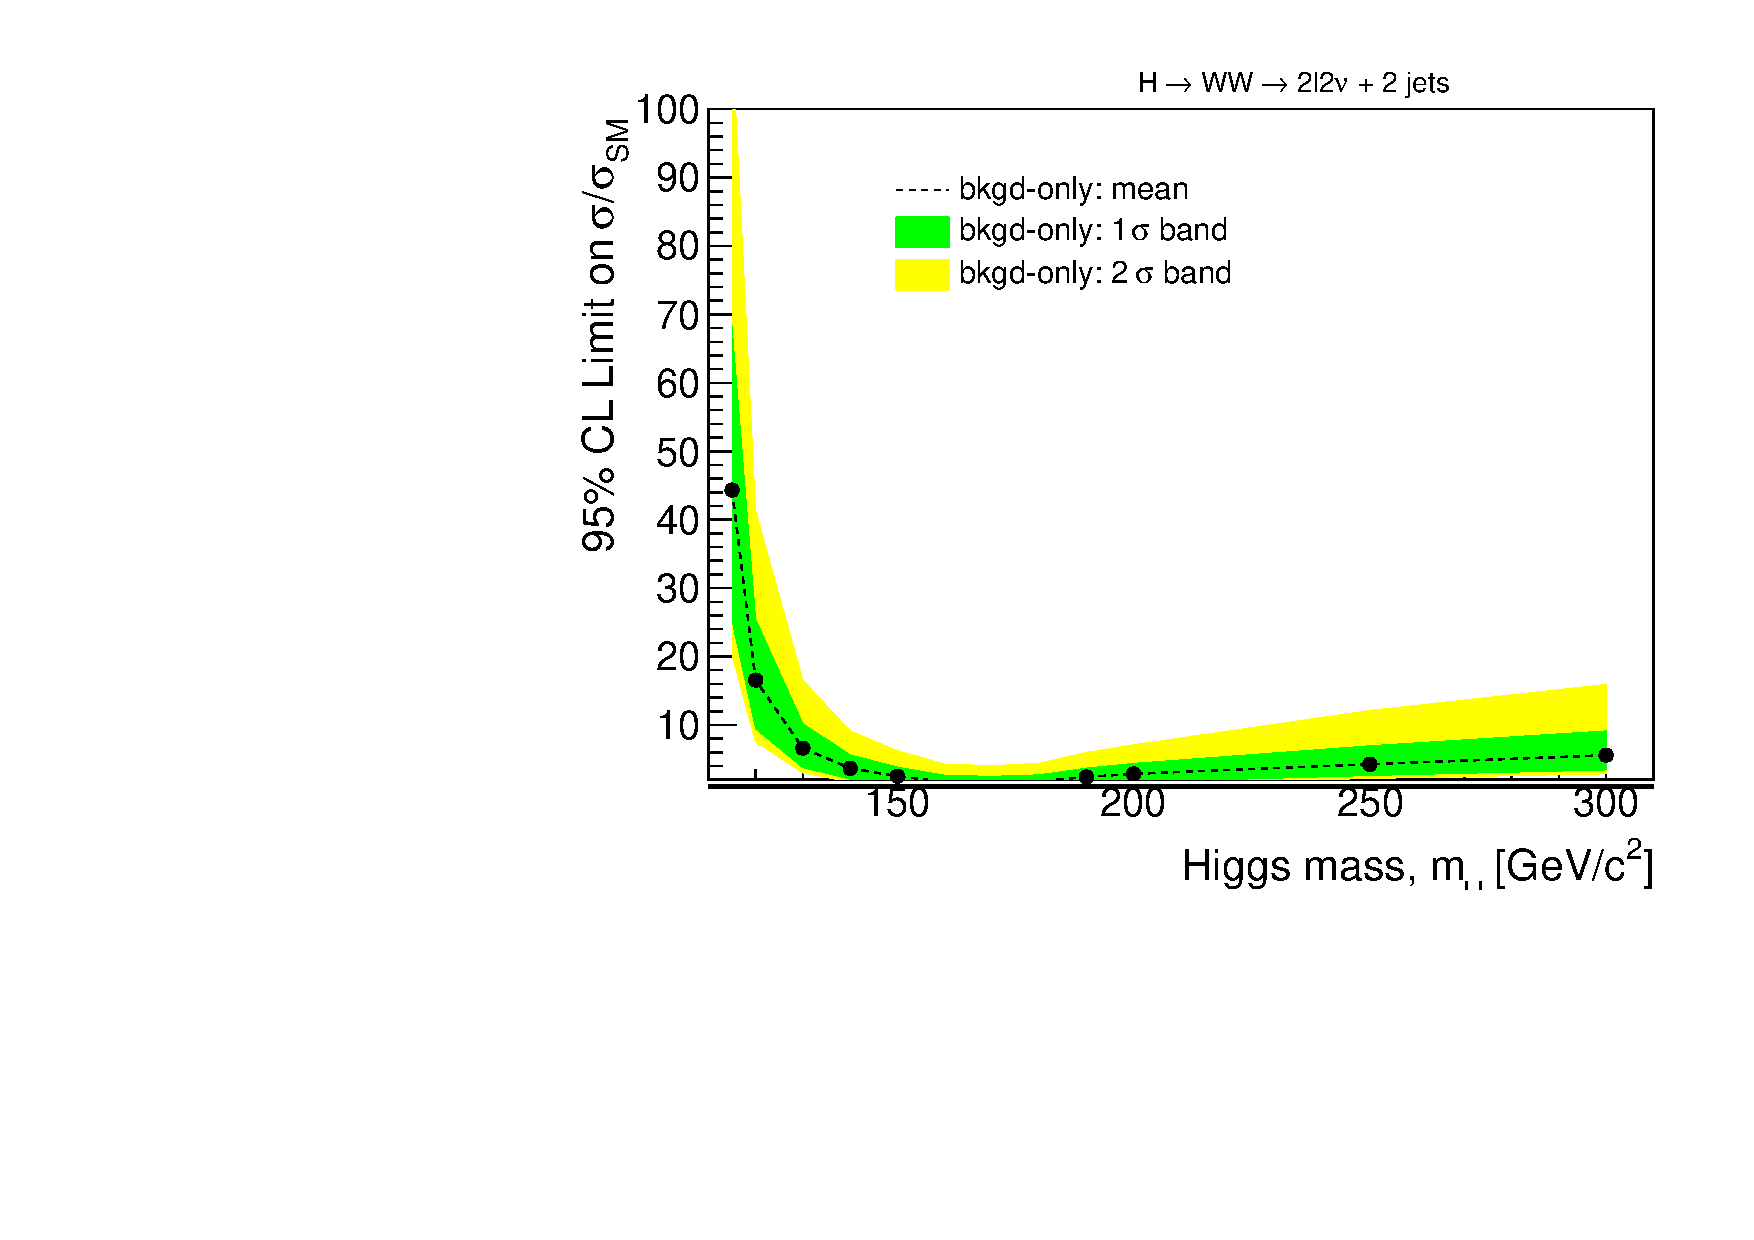
\includegraphics[width=0.49\textwidth]{figures/limits_2j_1000pb_cut_1.pdf}
   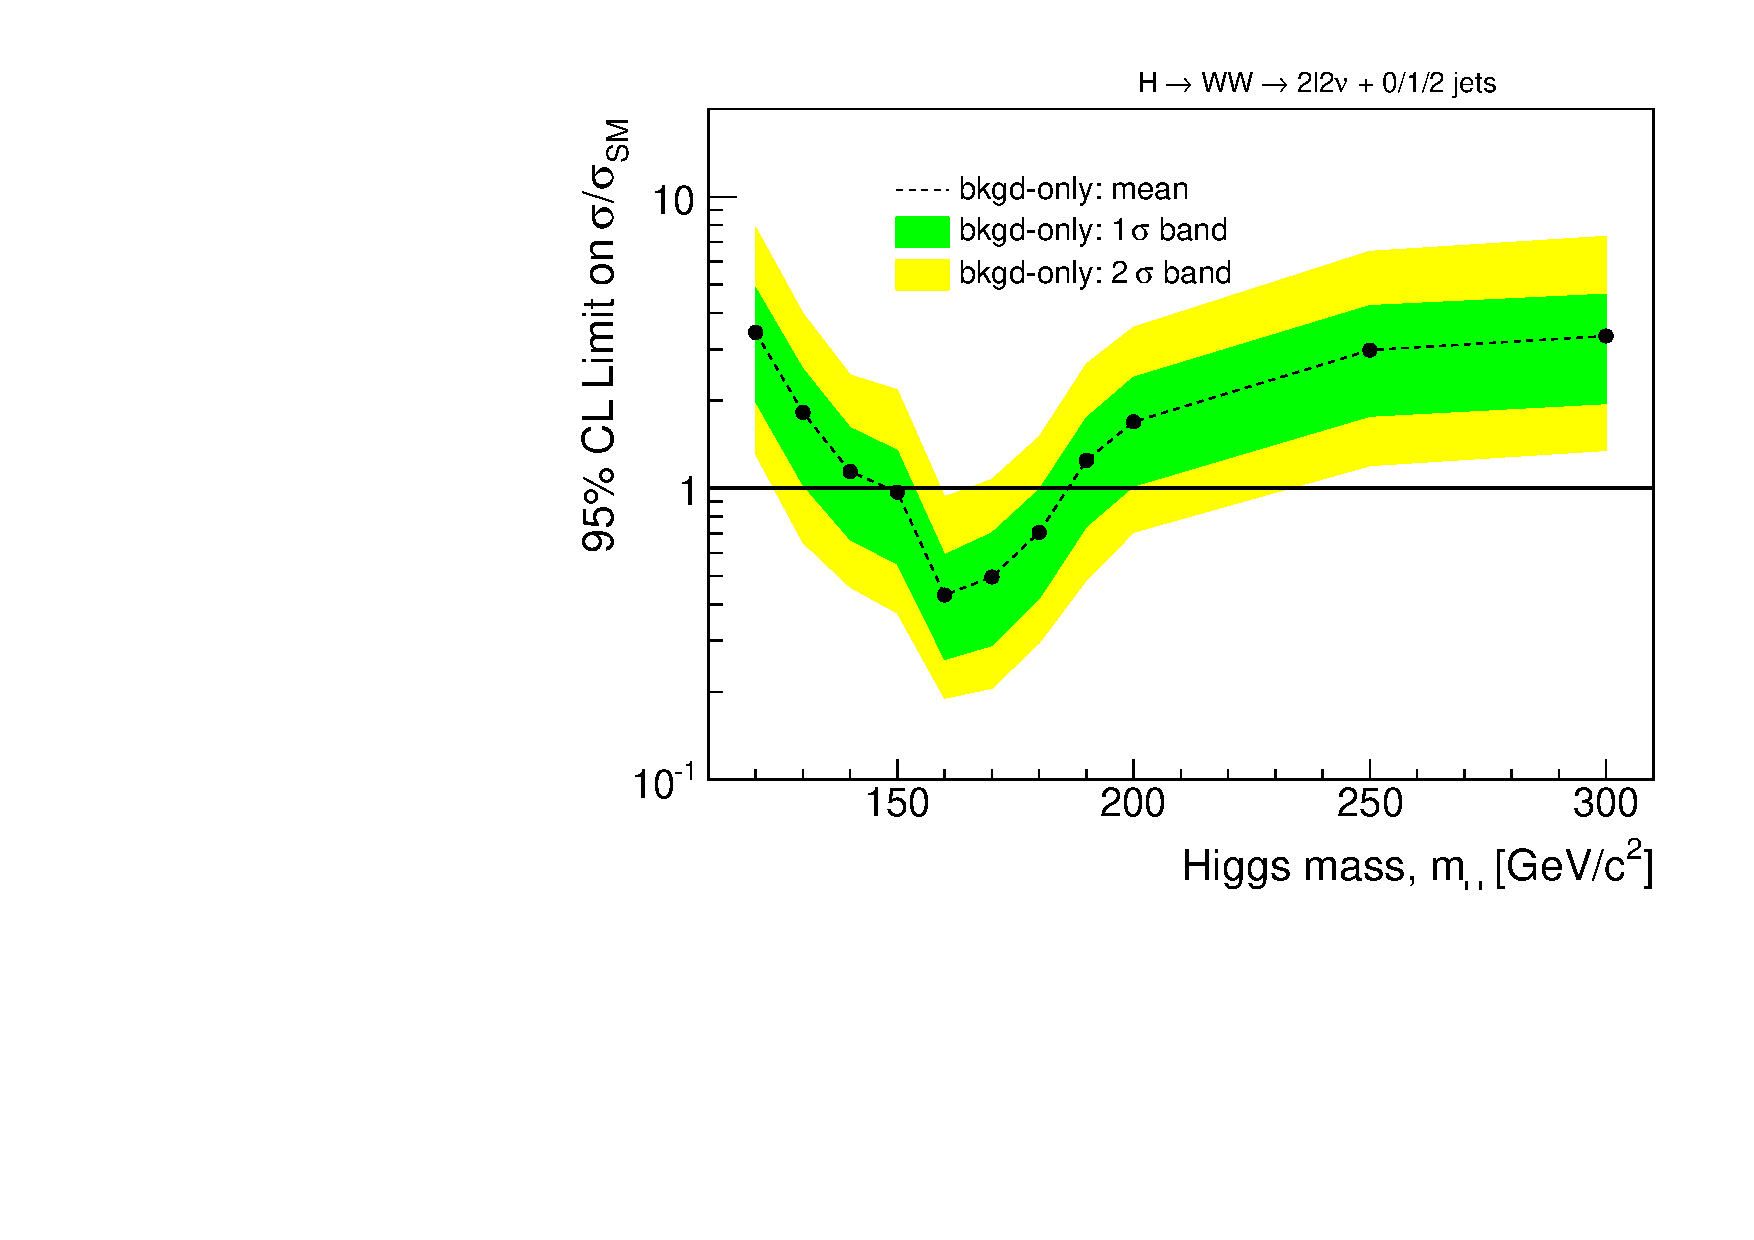
\includegraphics[width=0.49\textwidth]{figures/limits_nj_1000pb_cut_1.pdf}
   \caption{Cut based analysis expected upper limits at 95\% C.L. for 1\ifb\ of data. Top left plot 
   is the result for the 0-jet bin, top right plot is the result for the 1-jet bin, bottom left plot 
   is the result for the 2-jet bin and, bottom right plot is the combined result. The ``observed" limits 
   are just a simple toy Monte Carlo experiment.}
   \label{fig:cutbase_uls}
\end{center}
\end{figure}

\begin{figure}[!htbp]
\begin{center}
   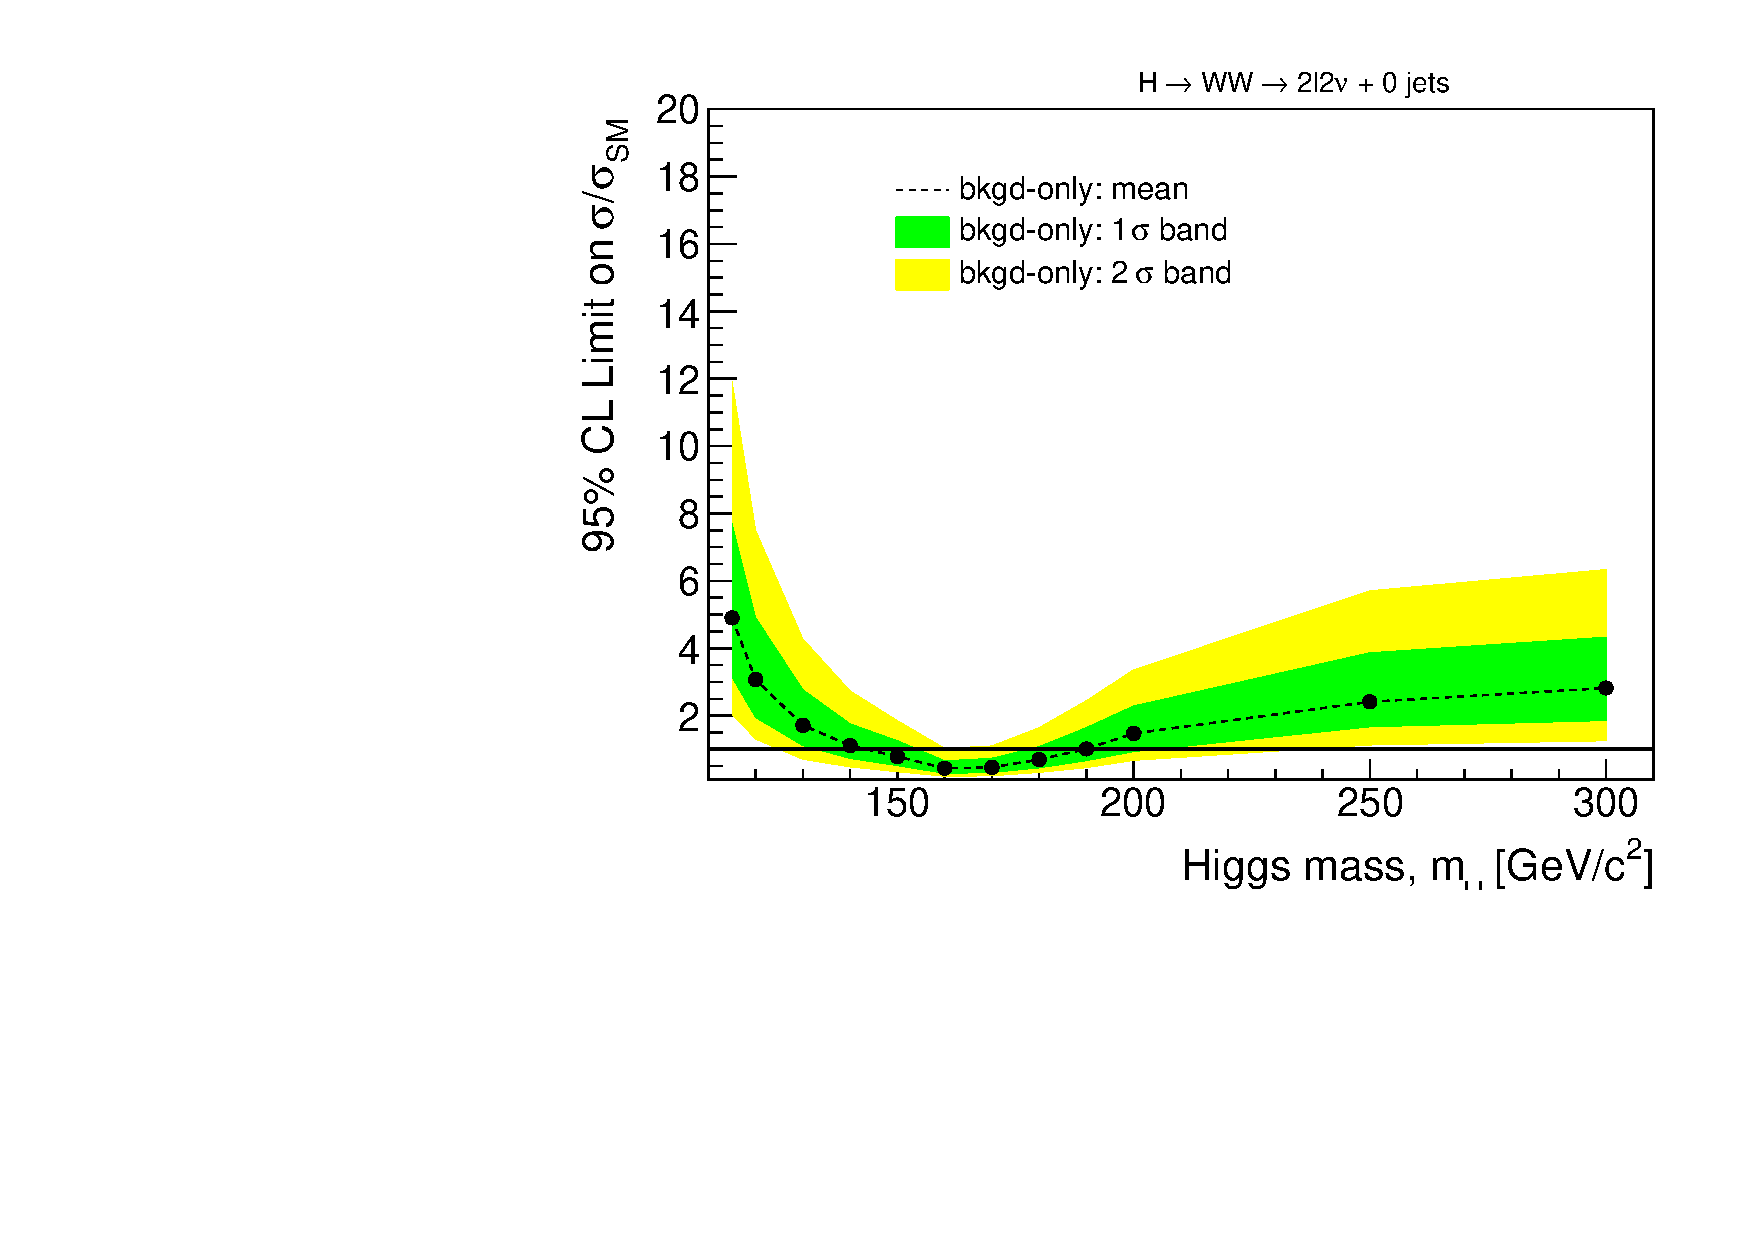
\includegraphics[width=0.49\textwidth]{figures/limits_0j_1000pb_mva_1.pdf}
   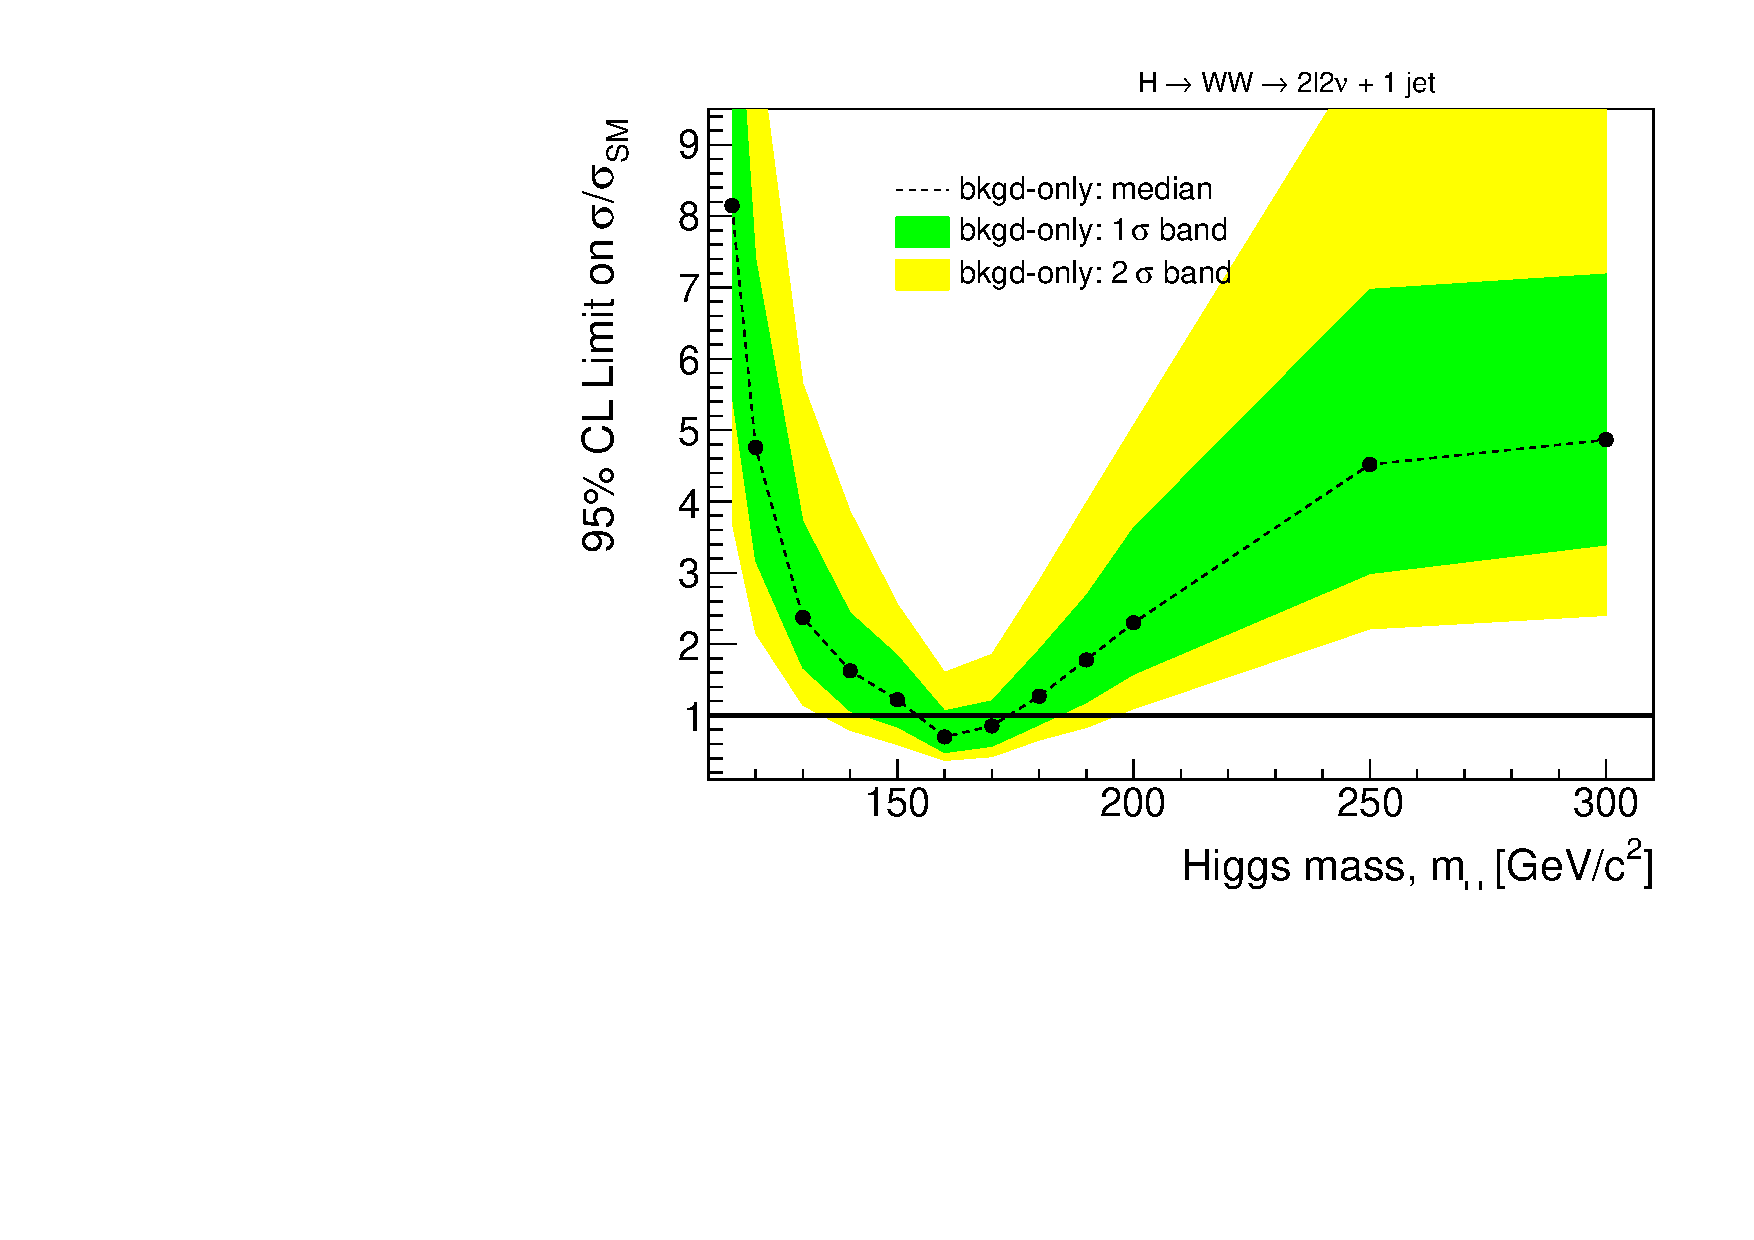
\includegraphics[width=0.49\textwidth]{figures/limits_1j_1000pb_mva_1.pdf}
   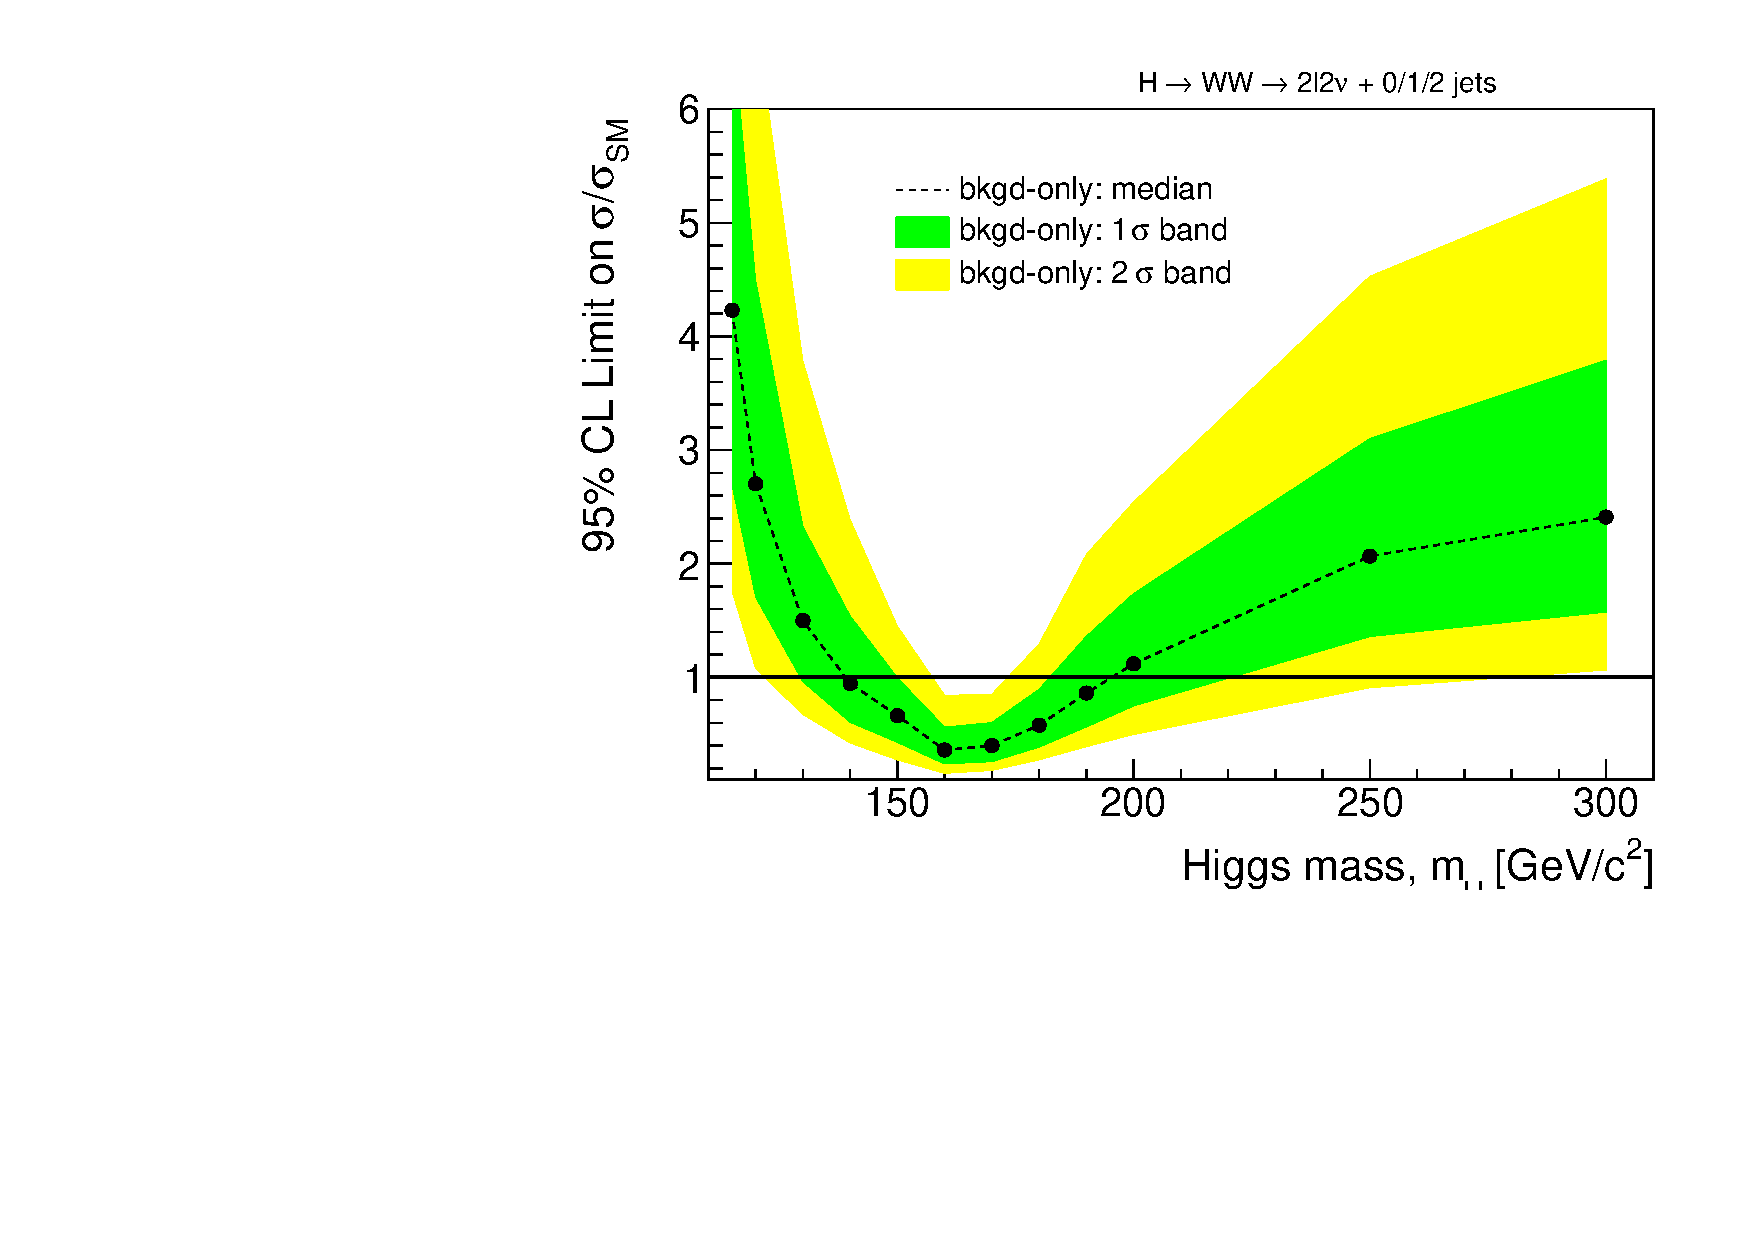
\includegraphics[width=0.49\textwidth]{figures/limits_nj_1000pb_mva_1.pdf}
   \caption{Multivariate cut-based analysis expected upper limits at 95\% C.L. for 1\ifb\ of data. Top left plot 
   is the result for the 0-jet bin, top right plot is the result for the 1-jet bin, and 
   bottom plot is the combined result including the cut based 2-jet bin analysis. The ``observed" limits 
   are just a simple toy Monte Carlo experiment.}
   \label{fig:mvabase_uls}
\end{center}
\end{figure}

\begin{figure}[!htbp]
\begin{center}
   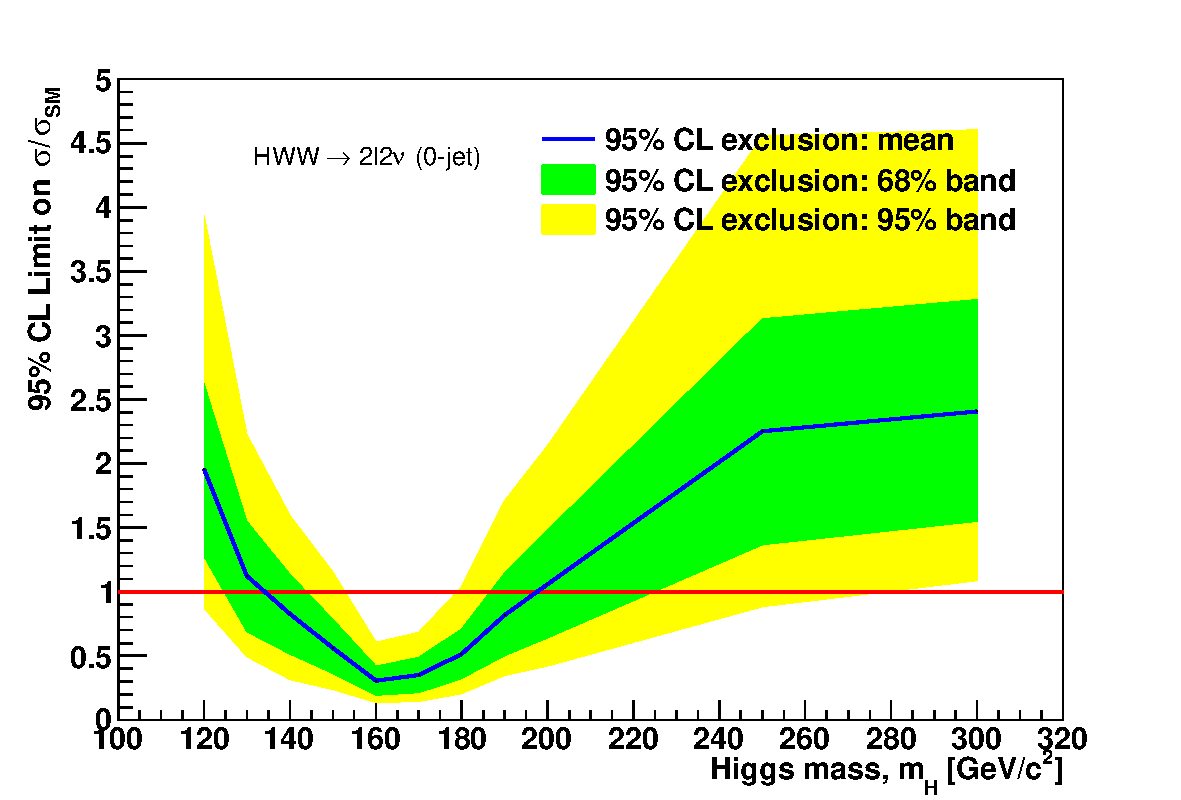
\includegraphics[width=0.49\textwidth]{figures/limits_mva_shape_1ifb_0jet.pdf}
   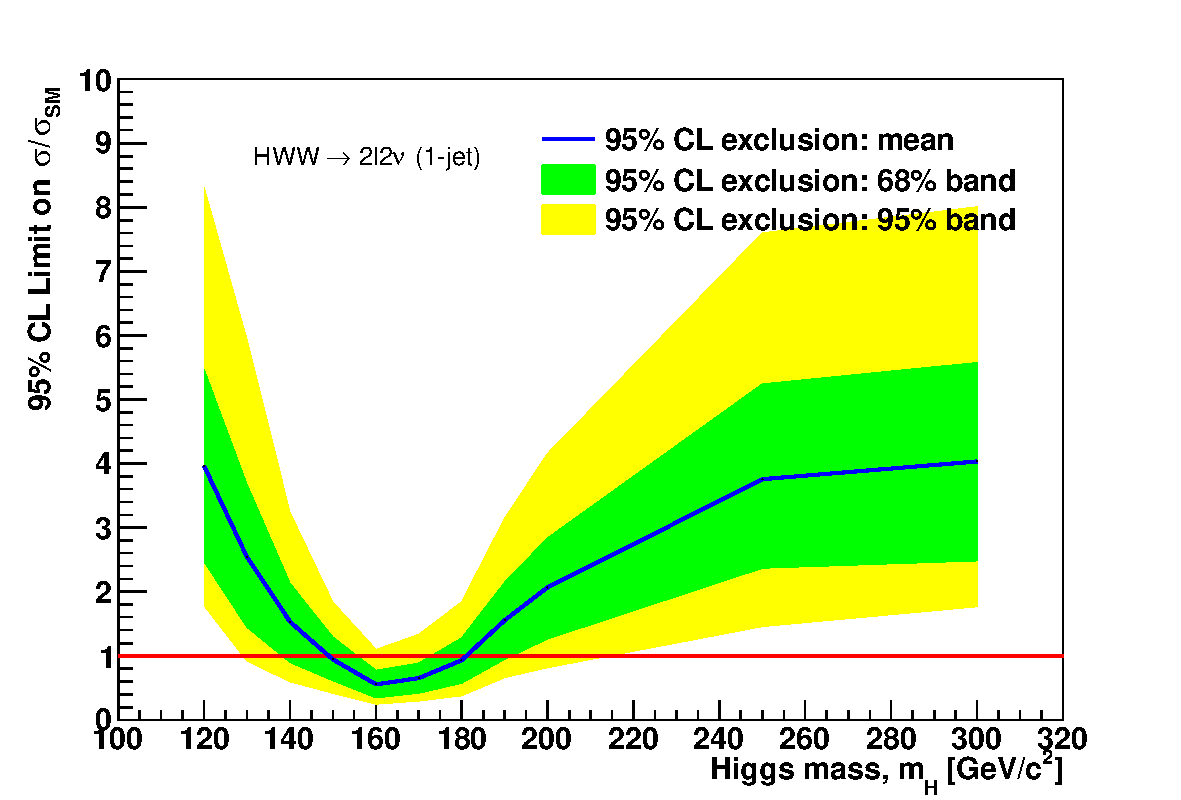
\includegraphics[width=0.49\textwidth]{figures/limits_mva_shape_1ifb_1jet.pdf}
   \caption{Multivariate shape analysis expected upper limits at 95\% C.L. for 1\ifb\ of data. Top left plot 
   is the result for the 0-jet bin, top right plot is the result for the 1-jet bin, and 
   bottom plot is the combined result including the cut based 2-jet bin analysis.}
   \label{fig:mvashape_uls}
\end{center}
\end{figure}
